\documentclass[twoside]{book}

% Packages required by doxygen
\usepackage{fixltx2e}
\usepackage{calc}
\usepackage{doxygen}
\usepackage[export]{adjustbox} % also loads graphicx
\usepackage{graphicx}
\usepackage[utf8]{inputenc}
\usepackage{makeidx}
\usepackage{multicol}
\usepackage{multirow}
\PassOptionsToPackage{warn}{textcomp}
\usepackage{textcomp}
\usepackage[nointegrals]{wasysym}
\usepackage[table]{xcolor}

% Font selection
\usepackage[T1]{fontenc}
\usepackage[scaled=.90]{helvet}
\usepackage{courier}
\usepackage{amssymb}
\usepackage{sectsty}
\renewcommand{\familydefault}{\sfdefault}
\allsectionsfont{%
  \fontseries{bc}\selectfont%
  \color{darkgray}%
}
\renewcommand{\DoxyLabelFont}{%
  \fontseries{bc}\selectfont%
  \color{darkgray}%
}
\newcommand{\+}{\discretionary{\mbox{\scriptsize$\hookleftarrow$}}{}{}}

% Page & text layout
\usepackage{geometry}
\geometry{%
  a4paper,%
  top=2.5cm,%
  bottom=2.5cm,%
  left=2.5cm,%
  right=2.5cm%
}
\tolerance=750
\hfuzz=15pt
\hbadness=750
\setlength{\emergencystretch}{15pt}
\setlength{\parindent}{0cm}
\setlength{\parskip}{3ex plus 2ex minus 2ex}
\makeatletter
\renewcommand{\paragraph}{%
  \@startsection{paragraph}{4}{0ex}{-1.0ex}{1.0ex}{%
    \normalfont\normalsize\bfseries\SS@parafont%
  }%
}
\renewcommand{\subparagraph}{%
  \@startsection{subparagraph}{5}{0ex}{-1.0ex}{1.0ex}{%
    \normalfont\normalsize\bfseries\SS@subparafont%
  }%
}
\makeatother

% Headers & footers
\usepackage{fancyhdr}
\pagestyle{fancyplain}
\fancyhead[LE]{\fancyplain{}{\bfseries\thepage}}
\fancyhead[CE]{\fancyplain{}{}}
\fancyhead[RE]{\fancyplain{}{\bfseries\leftmark}}
\fancyhead[LO]{\fancyplain{}{\bfseries\rightmark}}
\fancyhead[CO]{\fancyplain{}{}}
\fancyhead[RO]{\fancyplain{}{\bfseries\thepage}}
\fancyfoot[LE]{\fancyplain{}{}}
\fancyfoot[CE]{\fancyplain{}{}}
\fancyfoot[RE]{\fancyplain{}{\bfseries\scriptsize Generated by Doxygen }}
\fancyfoot[LO]{\fancyplain{}{\bfseries\scriptsize Generated by Doxygen }}
\fancyfoot[CO]{\fancyplain{}{}}
\fancyfoot[RO]{\fancyplain{}{}}
\renewcommand{\footrulewidth}{0.4pt}
\renewcommand{\chaptermark}[1]{%
  \markboth{#1}{}%
}
\renewcommand{\sectionmark}[1]{%
  \markright{\thesection\ #1}%
}

% Indices & bibliography
\usepackage{natbib}
\usepackage[titles]{tocloft}
\setcounter{tocdepth}{3}
\setcounter{secnumdepth}{5}
\makeindex

% Hyperlinks (required, but should be loaded last)
\usepackage{ifpdf}
\ifpdf
  \usepackage[pdftex,pagebackref=true]{hyperref}
\else
  \usepackage[ps2pdf,pagebackref=true]{hyperref}
\fi
\hypersetup{%
  colorlinks=true,%
  linkcolor=blue,%
  citecolor=blue,%
  unicode%
}

% Custom commands
\newcommand{\clearemptydoublepage}{%
  \newpage{\pagestyle{empty}\cleardoublepage}%
}

\usepackage{caption}
\captionsetup{labelsep=space,justification=centering,font={bf},singlelinecheck=off,skip=4pt,position=top}

%===== C O N T E N T S =====

\begin{document}

% Titlepage & ToC
\hypersetup{pageanchor=false,
             bookmarksnumbered=true,
             pdfencoding=unicode
            }
\pagenumbering{alph}
\begin{titlepage}
\vspace*{7cm}
\begin{center}%
{\Large P\+C\+S\+C2017\+\_\+\+Group2 }\\
\vspace*{1cm}
{\large Generated by Doxygen 1.8.13}\\
\end{center}
\end{titlepage}
\clearemptydoublepage
\pagenumbering{roman}
\tableofcontents
\clearemptydoublepage
\pagenumbering{arabic}
\hypersetup{pageanchor=true}

%--- Begin generated contents ---
\chapter{P\+C\+S\+C2017\+\_\+\+Group2}
\label{md__home_pcsc__p_c_s_c2017__group2__r_e_a_d_m_e}
\Hypertarget{md__home_pcsc__p_c_s_c2017__group2__r_e_a_d_m_e}
Monte Carlo 
\chapter{Hierarchical Index}
\section{Class Hierarchy}
This inheritance list is sorted roughly, but not completely, alphabetically\+:\begin{DoxyCompactList}
\item \contentsline{section}{Abstract\+Integrator}{\pageref{class_abstract_integrator}}{}
\begin{DoxyCompactList}
\item \contentsline{section}{Monte\+Carlo\+\_\+\+Metropolis\+Algorithm}{\pageref{class_monte_carlo___metropolis_algorithm}}{}
\item \contentsline{section}{Monte\+Carlo\+\_\+\+Uniform\+Sampling}{\pageref{class_monte_carlo___uniform_sampling}}{}
\end{DoxyCompactList}
\end{DoxyCompactList}

\chapter{Class Index}
\section{Class List}
Here are the classes, structs, unions and interfaces with brief descriptions\+:\begin{DoxyCompactList}
\item\contentsline{section}{\hyperlink{class_abstract_integrator}{Abstract\+Integrator} \\*An abstract class for setting the general inputs of an integral }{\pageref{class_abstract_integrator}}{}
\item\contentsline{section}{\hyperlink{class_monte_carlo___metropolis_algorithm}{Monte\+Carlo\+\_\+\+Metropolis\+Algorithm} \\*This class integrates a function using Metropolis sampling Brief description continued }{\pageref{class_monte_carlo___metropolis_algorithm}}{}
\item\contentsline{section}{\hyperlink{class_monte_carlo___uniform_sampling}{Monte\+Carlo\+\_\+\+Uniform\+Sampling} \\*This class integrates a function using uniform sampling }{\pageref{class_monte_carlo___uniform_sampling}}{}
\end{DoxyCompactList}

\chapter{File Index}
\section{File List}
Here is a list of all files with brief descriptions\+:\begin{DoxyCompactList}
\item\contentsline{section}{/home/pcsc/\+P\+C\+S\+C2017\+\_\+\+Group2/\hyperlink{_abstract_integrator_8cpp}{Abstract\+Integrator.\+cpp} }{\pageref{_abstract_integrator_8cpp}}{}
\item\contentsline{section}{/home/pcsc/\+P\+C\+S\+C2017\+\_\+\+Group2/\hyperlink{_abstract_integrator_8h}{Abstract\+Integrator.\+h} }{\pageref{_abstract_integrator_8h}}{}
\item\contentsline{section}{/home/pcsc/\+P\+C\+S\+C2017\+\_\+\+Group2/\hyperlink{main_8cpp}{main.\+cpp} }{\pageref{main_8cpp}}{}
\item\contentsline{section}{/home/pcsc/\+P\+C\+S\+C2017\+\_\+\+Group2/\hyperlink{_monte_carlo___metropolis_algorithm_8cpp}{Monte\+Carlo\+\_\+\+Metropolis\+Algorithm.\+cpp} }{\pageref{_monte_carlo___metropolis_algorithm_8cpp}}{}
\item\contentsline{section}{/home/pcsc/\+P\+C\+S\+C2017\+\_\+\+Group2/\hyperlink{_monte_carlo___metropolis_algorithm_8h}{Monte\+Carlo\+\_\+\+Metropolis\+Algorithm.\+h} }{\pageref{_monte_carlo___metropolis_algorithm_8h}}{}
\item\contentsline{section}{/home/pcsc/\+P\+C\+S\+C2017\+\_\+\+Group2/\hyperlink{_monte_carlo___uniform_sampling_8cpp}{Monte\+Carlo\+\_\+\+Uniform\+Sampling.\+cpp} }{\pageref{_monte_carlo___uniform_sampling_8cpp}}{}
\item\contentsline{section}{/home/pcsc/\+P\+C\+S\+C2017\+\_\+\+Group2/\hyperlink{_monte_carlo___uniform_sampling_8h}{Monte\+Carlo\+\_\+\+Uniform\+Sampling.\+h} }{\pageref{_monte_carlo___uniform_sampling_8h}}{}
\end{DoxyCompactList}

\chapter{Class Documentation}
\hypertarget{class_abstract_integrator}{}\section{Abstract\+Integrator Class Reference}
\label{class_abstract_integrator}\index{Abstract\+Integrator@{Abstract\+Integrator}}


An abstract class for setting the general inputs of an integral.  




{\ttfamily \#include $<$Abstract\+Integrator.\+h$>$}



Inheritance diagram for Abstract\+Integrator\+:\nopagebreak
\begin{figure}[H]
\begin{center}
\leavevmode
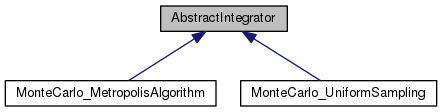
\includegraphics[width=350pt]{class_abstract_integrator__inherit__graph}
\end{center}
\end{figure}
\subsection*{Public Member Functions}
\begin{DoxyCompactItemize}
\item 
\hyperlink{class_abstract_integrator_aa88168bae2057a179c9ecc2ba9639f61}{Abstract\+Integrator} ()
\begin{DoxyCompactList}\small\item\em Constructor. \end{DoxyCompactList}\item 
virtual \hyperlink{class_abstract_integrator_addc528450d3f1d6e5d2cbd81e7d545e0}{$\sim$\+Abstract\+Integrator} ()
\begin{DoxyCompactList}\small\item\em Destructor. \end{DoxyCompactList}\item 
void \hyperlink{class_abstract_integrator_aea1949bda48ee6f4501475e8da26aaeb}{Set\+Lower\+Limit} (const double a)
\begin{DoxyCompactList}\small\item\em A method for setting the lower limit of integral by the user. \end{DoxyCompactList}\item 
void \hyperlink{class_abstract_integrator_a341070bf2dca9e2ac113d388e6d06556}{Set\+Upper\+Limit} (const double b)
\begin{DoxyCompactList}\small\item\em A method for setting the upper limit of integral by the user. \end{DoxyCompactList}\item 
void \hyperlink{class_abstract_integrator_a48c0b007c4b18e4a229f014bb0ccf9c0}{Set\+Sampling\+Number} (const int N)
\begin{DoxyCompactList}\small\item\em A method for setting the number of sampling in Monte-\/\+Carlo integration by the user. \end{DoxyCompactList}\item 
void \hyperlink{class_abstract_integrator_a9350f10f351d5b58c6aa8e581325ff4f}{Set\+Function} (double($\ast$\hyperlink{main_8cpp_a3de2b7b41a8e4b07da05298510d17ed2}{f})(double x))
\begin{DoxyCompactList}\small\item\em A method for setting the function by the user. \end{DoxyCompactList}\item 
void \hyperlink{class_abstract_integrator_a871fa27363ee09b98c964ccaa33da100}{Set\+Moment} (const int m)
\begin{DoxyCompactList}\small\item\em A method for setting the function by the user. \end{DoxyCompactList}\item 
double \hyperlink{class_abstract_integrator_ae27a09d1e3fb0a30ce9545a4d8f29cad}{Get\+Lower\+Limit} () const
\begin{DoxyCompactList}\small\item\em A method for getting the lower limit of integral. \end{DoxyCompactList}\item 
double \hyperlink{class_abstract_integrator_a864fe7dc9aa1ff0b36da0b8f361a5b69}{Get\+Upper\+Limit} () const
\begin{DoxyCompactList}\small\item\em A method for getting the upper limit of integral. \end{DoxyCompactList}\item 
int \hyperlink{class_abstract_integrator_ac58629ec6822b3beeefdd1323b627704}{Get\+Sampling\+Number} () const
\begin{DoxyCompactList}\small\item\em A method for getting the number of sampling. \end{DoxyCompactList}\item 
int \hyperlink{class_abstract_integrator_a7f709ab302dfe70b5f0f2ce80456fcdb}{Get\+Moment} () const
\begin{DoxyCompactList}\small\item\em A method for getting the moment. \end{DoxyCompactList}\item 
double \hyperlink{class_abstract_integrator_a6262731b81f3ad7e984ba354b4601356}{Function\+Value} (double x) const
\begin{DoxyCompactList}\small\item\em This method returns the value of function at the given input value (x) \end{DoxyCompactList}\item 
virtual double $\ast$ \hyperlink{class_abstract_integrator_a073d8f87239f732b3d2832070caa3b17}{Integrator} ()=0
\begin{DoxyCompactList}\small\item\em pure virtual method \end{DoxyCompactList}\end{DoxyCompactItemize}


\subsection{Detailed Description}
An abstract class for setting the general inputs of an integral. 

This class doesn\textquotesingle{}t include any numerical method for calculating the integral, rather, it has some methods used for setting the general inputs of an integral by the user and contains some members storing these inputs, which are used by numerical methods in the derived classes. 

Definition at line 13 of file Abstract\+Integrator.\+h.



\subsection{Constructor \& Destructor Documentation}
\mbox{\Hypertarget{class_abstract_integrator_aa88168bae2057a179c9ecc2ba9639f61}\label{class_abstract_integrator_aa88168bae2057a179c9ecc2ba9639f61}} 
\index{Abstract\+Integrator@{Abstract\+Integrator}!Abstract\+Integrator@{Abstract\+Integrator}}
\index{Abstract\+Integrator@{Abstract\+Integrator}!Abstract\+Integrator@{Abstract\+Integrator}}
\subsubsection{\texorpdfstring{Abstract\+Integrator()}{AbstractIntegrator()}}
{\footnotesize\ttfamily Abstract\+Integrator\+::\+Abstract\+Integrator (\begin{DoxyParamCaption}{ }\end{DoxyParamCaption})}



Constructor. 



Definition at line 7 of file Abstract\+Integrator.\+cpp.

\mbox{\Hypertarget{class_abstract_integrator_addc528450d3f1d6e5d2cbd81e7d545e0}\label{class_abstract_integrator_addc528450d3f1d6e5d2cbd81e7d545e0}} 
\index{Abstract\+Integrator@{Abstract\+Integrator}!````~Abstract\+Integrator@{$\sim$\+Abstract\+Integrator}}
\index{````~Abstract\+Integrator@{$\sim$\+Abstract\+Integrator}!Abstract\+Integrator@{Abstract\+Integrator}}
\subsubsection{\texorpdfstring{$\sim$\+Abstract\+Integrator()}{~AbstractIntegrator()}}
{\footnotesize\ttfamily Abstract\+Integrator\+::$\sim$\+Abstract\+Integrator (\begin{DoxyParamCaption}{ }\end{DoxyParamCaption})\hspace{0.3cm}{\ttfamily [virtual]}}



Destructor. 



Definition at line 8 of file Abstract\+Integrator.\+cpp.



\subsection{Member Function Documentation}
\mbox{\Hypertarget{class_abstract_integrator_a6262731b81f3ad7e984ba354b4601356}\label{class_abstract_integrator_a6262731b81f3ad7e984ba354b4601356}} 
\index{Abstract\+Integrator@{Abstract\+Integrator}!Function\+Value@{Function\+Value}}
\index{Function\+Value@{Function\+Value}!Abstract\+Integrator@{Abstract\+Integrator}}
\subsubsection{\texorpdfstring{Function\+Value()}{FunctionValue()}}
{\footnotesize\ttfamily double Abstract\+Integrator\+::\+Function\+Value (\begin{DoxyParamCaption}\item[{double}]{x }\end{DoxyParamCaption}) const}



This method returns the value of function at the given input value (x) 



Definition at line 76 of file Abstract\+Integrator.\+cpp.

\mbox{\Hypertarget{class_abstract_integrator_ae27a09d1e3fb0a30ce9545a4d8f29cad}\label{class_abstract_integrator_ae27a09d1e3fb0a30ce9545a4d8f29cad}} 
\index{Abstract\+Integrator@{Abstract\+Integrator}!Get\+Lower\+Limit@{Get\+Lower\+Limit}}
\index{Get\+Lower\+Limit@{Get\+Lower\+Limit}!Abstract\+Integrator@{Abstract\+Integrator}}
\subsubsection{\texorpdfstring{Get\+Lower\+Limit()}{GetLowerLimit()}}
{\footnotesize\ttfamily double Abstract\+Integrator\+::\+Get\+Lower\+Limit (\begin{DoxyParamCaption}{ }\end{DoxyParamCaption}) const}



A method for getting the lower limit of integral. 

This method is mainly used in some methods of derived classes, but it can also be called by the user. 

Definition at line 58 of file Abstract\+Integrator.\+cpp.

\mbox{\Hypertarget{class_abstract_integrator_a7f709ab302dfe70b5f0f2ce80456fcdb}\label{class_abstract_integrator_a7f709ab302dfe70b5f0f2ce80456fcdb}} 
\index{Abstract\+Integrator@{Abstract\+Integrator}!Get\+Moment@{Get\+Moment}}
\index{Get\+Moment@{Get\+Moment}!Abstract\+Integrator@{Abstract\+Integrator}}
\subsubsection{\texorpdfstring{Get\+Moment()}{GetMoment()}}
{\footnotesize\ttfamily int Abstract\+Integrator\+::\+Get\+Moment (\begin{DoxyParamCaption}{ }\end{DoxyParamCaption}) const}



A method for getting the moment. 

This method is mainly used in some methods of derived classes, but it can also be called by the user. 

Definition at line 70 of file Abstract\+Integrator.\+cpp.

\mbox{\Hypertarget{class_abstract_integrator_ac58629ec6822b3beeefdd1323b627704}\label{class_abstract_integrator_ac58629ec6822b3beeefdd1323b627704}} 
\index{Abstract\+Integrator@{Abstract\+Integrator}!Get\+Sampling\+Number@{Get\+Sampling\+Number}}
\index{Get\+Sampling\+Number@{Get\+Sampling\+Number}!Abstract\+Integrator@{Abstract\+Integrator}}
\subsubsection{\texorpdfstring{Get\+Sampling\+Number()}{GetSamplingNumber()}}
{\footnotesize\ttfamily int Abstract\+Integrator\+::\+Get\+Sampling\+Number (\begin{DoxyParamCaption}{ }\end{DoxyParamCaption}) const}



A method for getting the number of sampling. 

This method is mainly used in some methods of derived classes, but it can also be called by the user. 

Definition at line 66 of file Abstract\+Integrator.\+cpp.

\mbox{\Hypertarget{class_abstract_integrator_a864fe7dc9aa1ff0b36da0b8f361a5b69}\label{class_abstract_integrator_a864fe7dc9aa1ff0b36da0b8f361a5b69}} 
\index{Abstract\+Integrator@{Abstract\+Integrator}!Get\+Upper\+Limit@{Get\+Upper\+Limit}}
\index{Get\+Upper\+Limit@{Get\+Upper\+Limit}!Abstract\+Integrator@{Abstract\+Integrator}}
\subsubsection{\texorpdfstring{Get\+Upper\+Limit()}{GetUpperLimit()}}
{\footnotesize\ttfamily double Abstract\+Integrator\+::\+Get\+Upper\+Limit (\begin{DoxyParamCaption}{ }\end{DoxyParamCaption}) const}



A method for getting the upper limit of integral. 

This method is mainly used in some methods of derived classes, but it can also be called by the user. 

Definition at line 62 of file Abstract\+Integrator.\+cpp.

\mbox{\Hypertarget{class_abstract_integrator_a073d8f87239f732b3d2832070caa3b17}\label{class_abstract_integrator_a073d8f87239f732b3d2832070caa3b17}} 
\index{Abstract\+Integrator@{Abstract\+Integrator}!Integrator@{Integrator}}
\index{Integrator@{Integrator}!Abstract\+Integrator@{Abstract\+Integrator}}
\subsubsection{\texorpdfstring{Integrator()}{Integrator()}}
{\footnotesize\ttfamily virtual double$\ast$ Abstract\+Integrator\+::\+Integrator (\begin{DoxyParamCaption}{ }\end{DoxyParamCaption})\hspace{0.3cm}{\ttfamily [pure virtual]}}



pure virtual method 

in the derived classes, this method is overridden for implementing numerical algorithms 

Implemented in \hyperlink{class_monte_carlo___metropolis_algorithm_a93fba72a50330bf184156e23158992b2}{Monte\+Carlo\+\_\+\+Metropolis\+Algorithm}, and \hyperlink{class_monte_carlo___uniform_sampling_a1920387a9f817c8179531fa02f7c00d3}{Monte\+Carlo\+\_\+\+Uniform\+Sampling}.

\mbox{\Hypertarget{class_abstract_integrator_a9350f10f351d5b58c6aa8e581325ff4f}\label{class_abstract_integrator_a9350f10f351d5b58c6aa8e581325ff4f}} 
\index{Abstract\+Integrator@{Abstract\+Integrator}!Set\+Function@{Set\+Function}}
\index{Set\+Function@{Set\+Function}!Abstract\+Integrator@{Abstract\+Integrator}}
\subsubsection{\texorpdfstring{Set\+Function()}{SetFunction()}}
{\footnotesize\ttfamily void Abstract\+Integrator\+::\+Set\+Function (\begin{DoxyParamCaption}\item[{double($\ast$)(double x)}]{f }\end{DoxyParamCaption})}



A method for setting the function by the user. 



Definition at line 48 of file Abstract\+Integrator.\+cpp.

\mbox{\Hypertarget{class_abstract_integrator_aea1949bda48ee6f4501475e8da26aaeb}\label{class_abstract_integrator_aea1949bda48ee6f4501475e8da26aaeb}} 
\index{Abstract\+Integrator@{Abstract\+Integrator}!Set\+Lower\+Limit@{Set\+Lower\+Limit}}
\index{Set\+Lower\+Limit@{Set\+Lower\+Limit}!Abstract\+Integrator@{Abstract\+Integrator}}
\subsubsection{\texorpdfstring{Set\+Lower\+Limit()}{SetLowerLimit()}}
{\footnotesize\ttfamily void Abstract\+Integrator\+::\+Set\+Lower\+Limit (\begin{DoxyParamCaption}\item[{const double}]{a }\end{DoxyParamCaption})}



A method for setting the lower limit of integral by the user. 



Definition at line 12 of file Abstract\+Integrator.\+cpp.

\mbox{\Hypertarget{class_abstract_integrator_a871fa27363ee09b98c964ccaa33da100}\label{class_abstract_integrator_a871fa27363ee09b98c964ccaa33da100}} 
\index{Abstract\+Integrator@{Abstract\+Integrator}!Set\+Moment@{Set\+Moment}}
\index{Set\+Moment@{Set\+Moment}!Abstract\+Integrator@{Abstract\+Integrator}}
\subsubsection{\texorpdfstring{Set\+Moment()}{SetMoment()}}
{\footnotesize\ttfamily void Abstract\+Integrator\+::\+Set\+Moment (\begin{DoxyParamCaption}\item[{const int}]{m }\end{DoxyParamCaption})}



A method for setting the function by the user. 

as the default value of Moment is 0, user may not call it 

Definition at line 52 of file Abstract\+Integrator.\+cpp.

\mbox{\Hypertarget{class_abstract_integrator_a48c0b007c4b18e4a229f014bb0ccf9c0}\label{class_abstract_integrator_a48c0b007c4b18e4a229f014bb0ccf9c0}} 
\index{Abstract\+Integrator@{Abstract\+Integrator}!Set\+Sampling\+Number@{Set\+Sampling\+Number}}
\index{Set\+Sampling\+Number@{Set\+Sampling\+Number}!Abstract\+Integrator@{Abstract\+Integrator}}
\subsubsection{\texorpdfstring{Set\+Sampling\+Number()}{SetSamplingNumber()}}
{\footnotesize\ttfamily void Abstract\+Integrator\+::\+Set\+Sampling\+Number (\begin{DoxyParamCaption}\item[{const int}]{N }\end{DoxyParamCaption})}



A method for setting the number of sampling in Monte-\/\+Carlo integration by the user. 



Definition at line 44 of file Abstract\+Integrator.\+cpp.

\mbox{\Hypertarget{class_abstract_integrator_a341070bf2dca9e2ac113d388e6d06556}\label{class_abstract_integrator_a341070bf2dca9e2ac113d388e6d06556}} 
\index{Abstract\+Integrator@{Abstract\+Integrator}!Set\+Upper\+Limit@{Set\+Upper\+Limit}}
\index{Set\+Upper\+Limit@{Set\+Upper\+Limit}!Abstract\+Integrator@{Abstract\+Integrator}}
\subsubsection{\texorpdfstring{Set\+Upper\+Limit()}{SetUpperLimit()}}
{\footnotesize\ttfamily void Abstract\+Integrator\+::\+Set\+Upper\+Limit (\begin{DoxyParamCaption}\item[{const double}]{b }\end{DoxyParamCaption})}



A method for setting the upper limit of integral by the user. 



Definition at line 28 of file Abstract\+Integrator.\+cpp.



The documentation for this class was generated from the following files\+:\begin{DoxyCompactItemize}
\item 
\hyperlink{_abstract_integrator_8h}{Abstract\+Integrator.\+h}\item 
\hyperlink{_abstract_integrator_8cpp}{Abstract\+Integrator.\+cpp}\end{DoxyCompactItemize}

\hypertarget{class_monte_carlo___metropolis_algorithm}{}\section{Monte\+Carlo\+\_\+\+Metropolis\+Algorithm Class Reference}
\label{class_monte_carlo___metropolis_algorithm}\index{Monte\+Carlo\+\_\+\+Metropolis\+Algorithm@{Monte\+Carlo\+\_\+\+Metropolis\+Algorithm}}


This class integrates a function using Metropolis sampling.  




{\ttfamily \#include $<$Monte\+Carlo\+\_\+\+Metropolis\+Algorithm.\+h$>$}



Inheritance diagram for Monte\+Carlo\+\_\+\+Metropolis\+Algorithm\+:\nopagebreak
\begin{figure}[H]
\begin{center}
\leavevmode
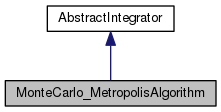
\includegraphics[width=238pt]{class_monte_carlo___metropolis_algorithm__inherit__graph}
\end{center}
\end{figure}


Collaboration diagram for Monte\+Carlo\+\_\+\+Metropolis\+Algorithm\+:\nopagebreak
\begin{figure}[H]
\begin{center}
\leavevmode
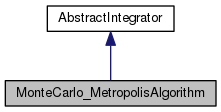
\includegraphics[width=238pt]{class_monte_carlo___metropolis_algorithm__coll__graph}
\end{center}
\end{figure}
\subsection*{Public Member Functions}
\begin{DoxyCompactItemize}
\item 
\hyperlink{class_monte_carlo___metropolis_algorithm_a80995ad029b056ca675c751c247426a5}{Monte\+Carlo\+\_\+\+Metropolis\+Algorithm} ()
\begin{DoxyCompactList}\small\item\em Constructor. \end{DoxyCompactList}\item 
\hyperlink{class_monte_carlo___metropolis_algorithm_aecedd40f8c0098bc66d455ef06814981}{$\sim$\+Monte\+Carlo\+\_\+\+Metropolis\+Algorithm} ()
\begin{DoxyCompactList}\small\item\em Destructor. \end{DoxyCompactList}\item 
void \hyperlink{class_monte_carlo___metropolis_algorithm_adcbfbdb6058a0a6de2f8b18698834a91}{Set\+Weight} (double($\ast$\hyperlink{main_8cpp_a6f95c347c46d0a26fc68408b470a98df}{w})(double x), bool flag=false)
\begin{DoxyCompactList}\small\item\em A method for setting the weight function by the user, flag=true if the function is normalized. \end{DoxyCompactList}\item 
double \hyperlink{class_monte_carlo___metropolis_algorithm_a5295f6e5691292d833da48105b13ece4}{Weight\+Value} (double x) const
\begin{DoxyCompactList}\small\item\em This method returns the value of weight function at the given input value (x) \end{DoxyCompactList}\item 
double $\ast$ \hyperlink{class_monte_carlo___metropolis_algorithm_a93fba72a50330bf184156e23158992b2}{Integrator} ()
\begin{DoxyCompactList}\small\item\em Integrating using Metropolis Algorithm. \end{DoxyCompactList}\end{DoxyCompactItemize}


\subsection{Detailed Description}
This class integrates a function using Metropolis sampling. 

In this method user must provide a strictly positive weight function on domain of integration. If the weight function is normalized, this method will perform integration and evaluates the error. If it is not the case, weight function will be normalized by integrating weight function on domain using Uniform Sampling class. The evaluation of error will consider the probable error in normalizing the weight function. The output is an array \char`\"{}ans\char`\"{} such that ans\mbox{[}0\mbox{]} is the integral answer and ans\mbox{[}1\mbox{]} is the estimated error. 

Definition at line 16 of file Monte\+Carlo\+\_\+\+Metropolis\+Algorithm.\+h.



\subsection{Constructor \& Destructor Documentation}
\mbox{\Hypertarget{class_monte_carlo___metropolis_algorithm_a80995ad029b056ca675c751c247426a5}\label{class_monte_carlo___metropolis_algorithm_a80995ad029b056ca675c751c247426a5}} 
\index{Monte\+Carlo\+\_\+\+Metropolis\+Algorithm@{Monte\+Carlo\+\_\+\+Metropolis\+Algorithm}!Monte\+Carlo\+\_\+\+Metropolis\+Algorithm@{Monte\+Carlo\+\_\+\+Metropolis\+Algorithm}}
\index{Monte\+Carlo\+\_\+\+Metropolis\+Algorithm@{Monte\+Carlo\+\_\+\+Metropolis\+Algorithm}!Monte\+Carlo\+\_\+\+Metropolis\+Algorithm@{Monte\+Carlo\+\_\+\+Metropolis\+Algorithm}}
\subsubsection{\texorpdfstring{Monte\+Carlo\+\_\+\+Metropolis\+Algorithm()}{MonteCarlo\_MetropolisAlgorithm()}}
{\footnotesize\ttfamily Monte\+Carlo\+\_\+\+Metropolis\+Algorithm\+::\+Monte\+Carlo\+\_\+\+Metropolis\+Algorithm (\begin{DoxyParamCaption}{ }\end{DoxyParamCaption})}



Constructor. 



Definition at line 13 of file Monte\+Carlo\+\_\+\+Metropolis\+Algorithm.\+cpp.

\mbox{\Hypertarget{class_monte_carlo___metropolis_algorithm_aecedd40f8c0098bc66d455ef06814981}\label{class_monte_carlo___metropolis_algorithm_aecedd40f8c0098bc66d455ef06814981}} 
\index{Monte\+Carlo\+\_\+\+Metropolis\+Algorithm@{Monte\+Carlo\+\_\+\+Metropolis\+Algorithm}!````~Monte\+Carlo\+\_\+\+Metropolis\+Algorithm@{$\sim$\+Monte\+Carlo\+\_\+\+Metropolis\+Algorithm}}
\index{````~Monte\+Carlo\+\_\+\+Metropolis\+Algorithm@{$\sim$\+Monte\+Carlo\+\_\+\+Metropolis\+Algorithm}!Monte\+Carlo\+\_\+\+Metropolis\+Algorithm@{Monte\+Carlo\+\_\+\+Metropolis\+Algorithm}}
\subsubsection{\texorpdfstring{$\sim$\+Monte\+Carlo\+\_\+\+Metropolis\+Algorithm()}{~MonteCarlo\_MetropolisAlgorithm()}}
{\footnotesize\ttfamily Monte\+Carlo\+\_\+\+Metropolis\+Algorithm\+::$\sim$\+Monte\+Carlo\+\_\+\+Metropolis\+Algorithm (\begin{DoxyParamCaption}{ }\end{DoxyParamCaption})}



Destructor. 



Definition at line 14 of file Monte\+Carlo\+\_\+\+Metropolis\+Algorithm.\+cpp.



\subsection{Member Function Documentation}
\mbox{\Hypertarget{class_monte_carlo___metropolis_algorithm_a93fba72a50330bf184156e23158992b2}\label{class_monte_carlo___metropolis_algorithm_a93fba72a50330bf184156e23158992b2}} 
\index{Monte\+Carlo\+\_\+\+Metropolis\+Algorithm@{Monte\+Carlo\+\_\+\+Metropolis\+Algorithm}!Integrator@{Integrator}}
\index{Integrator@{Integrator}!Monte\+Carlo\+\_\+\+Metropolis\+Algorithm@{Monte\+Carlo\+\_\+\+Metropolis\+Algorithm}}
\subsubsection{\texorpdfstring{Integrator()}{Integrator()}}
{\footnotesize\ttfamily double $\ast$ Monte\+Carlo\+\_\+\+Metropolis\+Algorithm\+::\+Integrator (\begin{DoxyParamCaption}{ }\end{DoxyParamCaption})\hspace{0.3cm}{\ttfamily [virtual]}}



Integrating using Metropolis Algorithm. 



Implements \hyperlink{class_abstract_integrator_a073d8f87239f732b3d2832070caa3b17}{Abstract\+Integrator}.



Definition at line 32 of file Monte\+Carlo\+\_\+\+Metropolis\+Algorithm.\+cpp.

\mbox{\Hypertarget{class_monte_carlo___metropolis_algorithm_adcbfbdb6058a0a6de2f8b18698834a91}\label{class_monte_carlo___metropolis_algorithm_adcbfbdb6058a0a6de2f8b18698834a91}} 
\index{Monte\+Carlo\+\_\+\+Metropolis\+Algorithm@{Monte\+Carlo\+\_\+\+Metropolis\+Algorithm}!Set\+Weight@{Set\+Weight}}
\index{Set\+Weight@{Set\+Weight}!Monte\+Carlo\+\_\+\+Metropolis\+Algorithm@{Monte\+Carlo\+\_\+\+Metropolis\+Algorithm}}
\subsubsection{\texorpdfstring{Set\+Weight()}{SetWeight()}}
{\footnotesize\ttfamily void Monte\+Carlo\+\_\+\+Metropolis\+Algorithm\+::\+Set\+Weight (\begin{DoxyParamCaption}\item[{double($\ast$)(double x)}]{w,  }\item[{bool}]{flag = {\ttfamily false} }\end{DoxyParamCaption})}



A method for setting the weight function by the user, flag=true if the function is normalized. 

the default Flag has been set false, so if the user doesn\textquotesingle{}t know whether his weight function is normalized or not, he can leave the second argument 

Definition at line 18 of file Monte\+Carlo\+\_\+\+Metropolis\+Algorithm.\+cpp.

\mbox{\Hypertarget{class_monte_carlo___metropolis_algorithm_a5295f6e5691292d833da48105b13ece4}\label{class_monte_carlo___metropolis_algorithm_a5295f6e5691292d833da48105b13ece4}} 
\index{Monte\+Carlo\+\_\+\+Metropolis\+Algorithm@{Monte\+Carlo\+\_\+\+Metropolis\+Algorithm}!Weight\+Value@{Weight\+Value}}
\index{Weight\+Value@{Weight\+Value}!Monte\+Carlo\+\_\+\+Metropolis\+Algorithm@{Monte\+Carlo\+\_\+\+Metropolis\+Algorithm}}
\subsubsection{\texorpdfstring{Weight\+Value()}{WeightValue()}}
{\footnotesize\ttfamily double Monte\+Carlo\+\_\+\+Metropolis\+Algorithm\+::\+Weight\+Value (\begin{DoxyParamCaption}\item[{double}]{x }\end{DoxyParamCaption}) const}



This method returns the value of weight function at the given input value (x) 



Definition at line 25 of file Monte\+Carlo\+\_\+\+Metropolis\+Algorithm.\+cpp.



The documentation for this class was generated from the following files\+:\begin{DoxyCompactItemize}
\item 
\hyperlink{_monte_carlo___metropolis_algorithm_8h}{Monte\+Carlo\+\_\+\+Metropolis\+Algorithm.\+h}\item 
\hyperlink{_monte_carlo___metropolis_algorithm_8cpp}{Monte\+Carlo\+\_\+\+Metropolis\+Algorithm.\+cpp}\end{DoxyCompactItemize}

\hypertarget{class_monte_carlo___uniform_sampling}{}\section{Monte\+Carlo\+\_\+\+Uniform\+Sampling Class Reference}
\label{class_monte_carlo___uniform_sampling}\index{Monte\+Carlo\+\_\+\+Uniform\+Sampling@{Monte\+Carlo\+\_\+\+Uniform\+Sampling}}


This class integrates a function using uniform sampling.  




{\ttfamily \#include $<$Monte\+Carlo\+\_\+\+Uniform\+Sampling.\+h$>$}



Inheritance diagram for Monte\+Carlo\+\_\+\+Uniform\+Sampling\+:\nopagebreak
\begin{figure}[H]
\begin{center}
\leavevmode
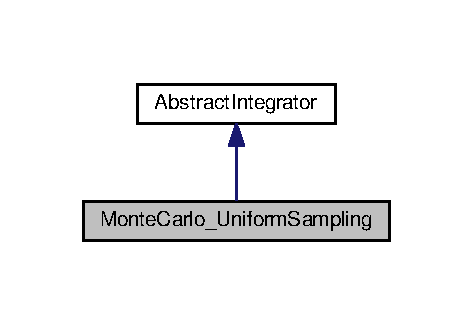
\includegraphics[width=227pt]{class_monte_carlo___uniform_sampling__inherit__graph}
\end{center}
\end{figure}


Collaboration diagram for Monte\+Carlo\+\_\+\+Uniform\+Sampling\+:\nopagebreak
\begin{figure}[H]
\begin{center}
\leavevmode
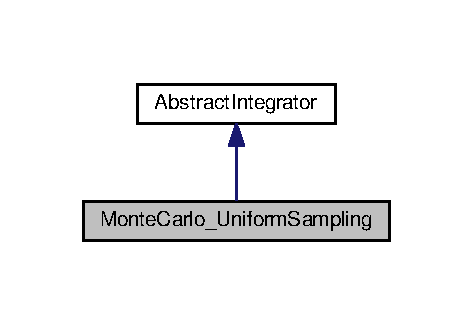
\includegraphics[width=227pt]{class_monte_carlo___uniform_sampling__coll__graph}
\end{center}
\end{figure}
\subsection*{Public Member Functions}
\begin{DoxyCompactItemize}
\item 
\hyperlink{class_monte_carlo___uniform_sampling_a1bf0ba8eb4f67d693a21e2d40601ee17}{Monte\+Carlo\+\_\+\+Uniform\+Sampling} ()
\begin{DoxyCompactList}\small\item\em Constructor. \end{DoxyCompactList}\item 
\hyperlink{class_monte_carlo___uniform_sampling_a1ccdb02604ffeb1f334b55ec24584f0c}{$\sim$\+Monte\+Carlo\+\_\+\+Uniform\+Sampling} ()
\begin{DoxyCompactList}\small\item\em Destructor. \end{DoxyCompactList}\item 
double $\ast$ \hyperlink{class_monte_carlo___uniform_sampling_a1920387a9f817c8179531fa02f7c00d3}{Integrator} ()
\begin{DoxyCompactList}\small\item\em Integrating using Uniform Sampling method. \end{DoxyCompactList}\end{DoxyCompactItemize}


\subsection{Detailed Description}
This class integrates a function using uniform sampling. 

In this method there is no need for weight function. Integral and the error would be evaluated directly. The output is an array \char`\"{}ans\char`\"{} such that ans\mbox{[}0\mbox{]} is the integral answer and ans\mbox{[}1\mbox{]} is the estimated error. 

Definition at line 13 of file Monte\+Carlo\+\_\+\+Uniform\+Sampling.\+h.



\subsection{Constructor \& Destructor Documentation}
\mbox{\Hypertarget{class_monte_carlo___uniform_sampling_a1bf0ba8eb4f67d693a21e2d40601ee17}\label{class_monte_carlo___uniform_sampling_a1bf0ba8eb4f67d693a21e2d40601ee17}} 
\index{Monte\+Carlo\+\_\+\+Uniform\+Sampling@{Monte\+Carlo\+\_\+\+Uniform\+Sampling}!Monte\+Carlo\+\_\+\+Uniform\+Sampling@{Monte\+Carlo\+\_\+\+Uniform\+Sampling}}
\index{Monte\+Carlo\+\_\+\+Uniform\+Sampling@{Monte\+Carlo\+\_\+\+Uniform\+Sampling}!Monte\+Carlo\+\_\+\+Uniform\+Sampling@{Monte\+Carlo\+\_\+\+Uniform\+Sampling}}
\subsubsection{\texorpdfstring{Monte\+Carlo\+\_\+\+Uniform\+Sampling()}{MonteCarlo\_UniformSampling()}}
{\footnotesize\ttfamily Monte\+Carlo\+\_\+\+Uniform\+Sampling\+::\+Monte\+Carlo\+\_\+\+Uniform\+Sampling (\begin{DoxyParamCaption}{ }\end{DoxyParamCaption})}



Constructor. 



Definition at line 12 of file Monte\+Carlo\+\_\+\+Uniform\+Sampling.\+cpp.

\mbox{\Hypertarget{class_monte_carlo___uniform_sampling_a1ccdb02604ffeb1f334b55ec24584f0c}\label{class_monte_carlo___uniform_sampling_a1ccdb02604ffeb1f334b55ec24584f0c}} 
\index{Monte\+Carlo\+\_\+\+Uniform\+Sampling@{Monte\+Carlo\+\_\+\+Uniform\+Sampling}!````~Monte\+Carlo\+\_\+\+Uniform\+Sampling@{$\sim$\+Monte\+Carlo\+\_\+\+Uniform\+Sampling}}
\index{````~Monte\+Carlo\+\_\+\+Uniform\+Sampling@{$\sim$\+Monte\+Carlo\+\_\+\+Uniform\+Sampling}!Monte\+Carlo\+\_\+\+Uniform\+Sampling@{Monte\+Carlo\+\_\+\+Uniform\+Sampling}}
\subsubsection{\texorpdfstring{$\sim$\+Monte\+Carlo\+\_\+\+Uniform\+Sampling()}{~MonteCarlo\_UniformSampling()}}
{\footnotesize\ttfamily Monte\+Carlo\+\_\+\+Uniform\+Sampling\+::$\sim$\+Monte\+Carlo\+\_\+\+Uniform\+Sampling (\begin{DoxyParamCaption}{ }\end{DoxyParamCaption})}



Destructor. 



Definition at line 13 of file Monte\+Carlo\+\_\+\+Uniform\+Sampling.\+cpp.



\subsection{Member Function Documentation}
\mbox{\Hypertarget{class_monte_carlo___uniform_sampling_a1920387a9f817c8179531fa02f7c00d3}\label{class_monte_carlo___uniform_sampling_a1920387a9f817c8179531fa02f7c00d3}} 
\index{Monte\+Carlo\+\_\+\+Uniform\+Sampling@{Monte\+Carlo\+\_\+\+Uniform\+Sampling}!Integrator@{Integrator}}
\index{Integrator@{Integrator}!Monte\+Carlo\+\_\+\+Uniform\+Sampling@{Monte\+Carlo\+\_\+\+Uniform\+Sampling}}
\subsubsection{\texorpdfstring{Integrator()}{Integrator()}}
{\footnotesize\ttfamily double $\ast$ Monte\+Carlo\+\_\+\+Uniform\+Sampling\+::\+Integrator (\begin{DoxyParamCaption}{ }\end{DoxyParamCaption})\hspace{0.3cm}{\ttfamily [virtual]}}



Integrating using Uniform Sampling method. 



Implements \hyperlink{class_abstract_integrator_a073d8f87239f732b3d2832070caa3b17}{Abstract\+Integrator}.



Definition at line 17 of file Monte\+Carlo\+\_\+\+Uniform\+Sampling.\+cpp.



The documentation for this class was generated from the following files\+:\begin{DoxyCompactItemize}
\item 
\hyperlink{_monte_carlo___uniform_sampling_8h}{Monte\+Carlo\+\_\+\+Uniform\+Sampling.\+h}\item 
\hyperlink{_monte_carlo___uniform_sampling_8cpp}{Monte\+Carlo\+\_\+\+Uniform\+Sampling.\+cpp}\end{DoxyCompactItemize}

\chapter{File Documentation}
\hypertarget{_abstract_integrator_8cpp}{}\section{Abstract\+Integrator.\+cpp File Reference}
\label{_abstract_integrator_8cpp}\index{Abstract\+Integrator.\+cpp@{Abstract\+Integrator.\+cpp}}
{\ttfamily \#include \char`\"{}Abstract\+Integrator.\+h\char`\"{}}\newline
Include dependency graph for Abstract\+Integrator.\+cpp\+:
\nopagebreak
\begin{figure}[H]
\begin{center}
\leavevmode
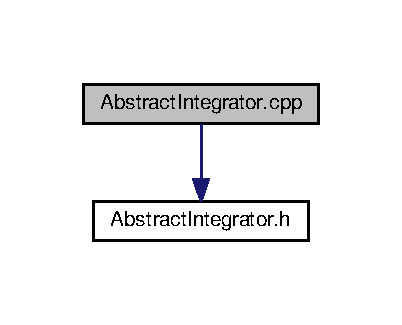
\includegraphics[width=193pt]{_abstract_integrator_8cpp__incl}
\end{center}
\end{figure}

\hypertarget{_abstract_integrator_8h}{}\section{/home/pcsc/\+P\+C\+S\+C2017\+\_\+\+Group2/\+Abstract\+Integrator.h File Reference}
\label{_abstract_integrator_8h}\index{/home/pcsc/\+P\+C\+S\+C2017\+\_\+\+Group2/\+Abstract\+Integrator.\+h@{/home/pcsc/\+P\+C\+S\+C2017\+\_\+\+Group2/\+Abstract\+Integrator.\+h}}
This graph shows which files directly or indirectly include this file\+:
% FIG 0
\subsection*{Classes}
\begin{DoxyCompactItemize}
\item 
class \hyperlink{class_abstract_integrator}{Abstract\+Integrator}
\begin{DoxyCompactList}\small\item\em An abstract class for setting the general inputs of an integral. \end{DoxyCompactList}\end{DoxyCompactItemize}

\hypertarget{main_8cpp}{}\section{main.\+cpp File Reference}
\label{main_8cpp}\index{main.\+cpp@{main.\+cpp}}
{\ttfamily \#include $<$iostream$>$}\newline
{\ttfamily \#include $<$cmath$>$}\newline
{\ttfamily \#include $<$iomanip$>$}\newline
{\ttfamily \#include \char`\"{}Abstract\+Integrator.\+h\char`\"{}}\newline
{\ttfamily \#include \char`\"{}Monte\+Carlo\+\_\+\+Uniform\+Sampling.\+h\char`\"{}}\newline
{\ttfamily \#include \char`\"{}Monte\+Carlo\+\_\+\+Metropolis\+Algorithm.\+h\char`\"{}}\newline
Include dependency graph for main.\+cpp\+:\nopagebreak
\begin{figure}[H]
\begin{center}
\leavevmode
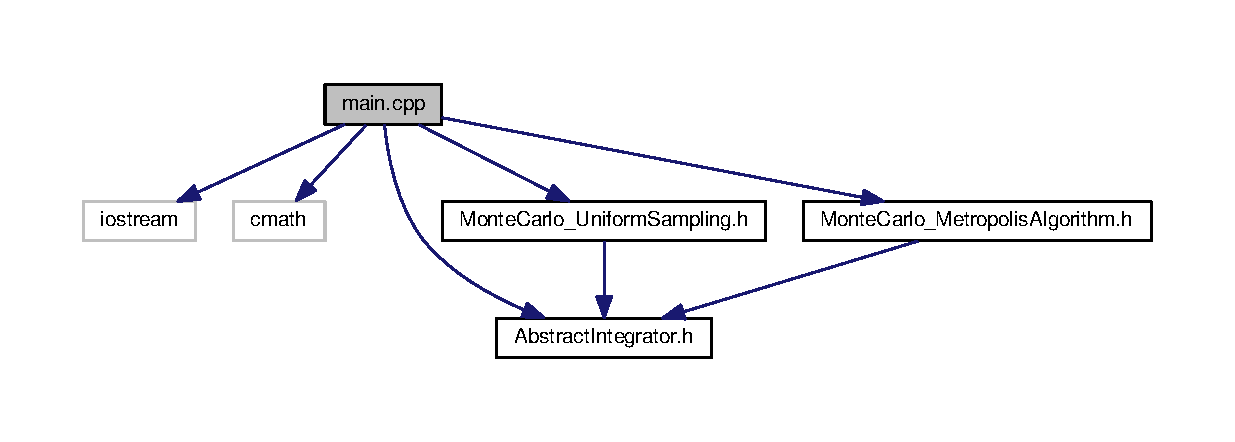
\includegraphics[width=350pt]{main_8cpp__incl}
\end{center}
\end{figure}
\subsection*{Functions}
\begin{DoxyCompactItemize}
\item 
double \hyperlink{main_8cpp_a3de2b7b41a8e4b07da05298510d17ed2}{f} (double x)
\item 
double \hyperlink{main_8cpp_a6f95c347c46d0a26fc68408b470a98df}{w} (double x)
\item 
int \hyperlink{main_8cpp_ae66f6b31b5ad750f1fe042a706a4e3d4}{main} ()
\end{DoxyCompactItemize}


\subsection{Function Documentation}
\mbox{\Hypertarget{main_8cpp_a3de2b7b41a8e4b07da05298510d17ed2}\label{main_8cpp_a3de2b7b41a8e4b07da05298510d17ed2}} 
\index{main.\+cpp@{main.\+cpp}!f@{f}}
\index{f@{f}!main.\+cpp@{main.\+cpp}}
\subsubsection{\texorpdfstring{f()}{f()}}
{\footnotesize\ttfamily double f (\begin{DoxyParamCaption}\item[{double}]{x }\end{DoxyParamCaption})}



Definition at line 9 of file main.\+cpp.

\mbox{\Hypertarget{main_8cpp_ae66f6b31b5ad750f1fe042a706a4e3d4}\label{main_8cpp_ae66f6b31b5ad750f1fe042a706a4e3d4}} 
\index{main.\+cpp@{main.\+cpp}!main@{main}}
\index{main@{main}!main.\+cpp@{main.\+cpp}}
\subsubsection{\texorpdfstring{main()}{main()}}
{\footnotesize\ttfamily int main (\begin{DoxyParamCaption}{ }\end{DoxyParamCaption})}



Definition at line 19 of file main.\+cpp.

\mbox{\Hypertarget{main_8cpp_a6f95c347c46d0a26fc68408b470a98df}\label{main_8cpp_a6f95c347c46d0a26fc68408b470a98df}} 
\index{main.\+cpp@{main.\+cpp}!w@{w}}
\index{w@{w}!main.\+cpp@{main.\+cpp}}
\subsubsection{\texorpdfstring{w()}{w()}}
{\footnotesize\ttfamily double w (\begin{DoxyParamCaption}\item[{double}]{x }\end{DoxyParamCaption})}



Definition at line 14 of file main.\+cpp.


\hypertarget{_monte_carlo___metropolis_algorithm_8cpp}{}\section{/home/pcsc/\+P\+C\+S\+C2017\+\_\+\+Group2/\+Monte\+Carlo\+\_\+\+Metropolis\+Algorithm.cpp File Reference}
\label{_monte_carlo___metropolis_algorithm_8cpp}\index{/home/pcsc/\+P\+C\+S\+C2017\+\_\+\+Group2/\+Monte\+Carlo\+\_\+\+Metropolis\+Algorithm.\+cpp@{/home/pcsc/\+P\+C\+S\+C2017\+\_\+\+Group2/\+Monte\+Carlo\+\_\+\+Metropolis\+Algorithm.\+cpp}}
{\ttfamily \#include \char`\"{}Monte\+Carlo\+\_\+\+Metropolis\+Algorithm.\+h\char`\"{}}\newline
{\ttfamily \#include $<$cmath$>$}\newline
{\ttfamily \#include $<$cstdlib$>$}\newline
{\ttfamily \#include $<$ctime$>$}\newline
{\ttfamily \#include $<$iostream$>$}\newline
{\ttfamily \#include $<$random$>$}\newline
{\ttfamily \#include $<$chrono$>$}\newline
Include dependency graph for Monte\+Carlo\+\_\+\+Metropolis\+Algorithm.\+cpp\+:
% FIG 0

\hypertarget{_monte_carlo___metropolis_algorithm_8h}{}\section{Monte\+Carlo\+\_\+\+Metropolis\+Algorithm.\+h File Reference}
\label{_monte_carlo___metropolis_algorithm_8h}\index{Monte\+Carlo\+\_\+\+Metropolis\+Algorithm.\+h@{Monte\+Carlo\+\_\+\+Metropolis\+Algorithm.\+h}}
{\ttfamily \#include \char`\"{}Abstract\+Integrator.\+h\char`\"{}}\newline
Include dependency graph for Monte\+Carlo\+\_\+\+Metropolis\+Algorithm.\+h\+:
\nopagebreak
\begin{figure}[H]
\begin{center}
\leavevmode
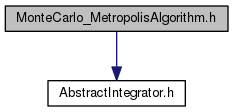
\includegraphics[width=247pt]{_monte_carlo___metropolis_algorithm_8h__incl}
\end{center}
\end{figure}
This graph shows which files directly or indirectly include this file\+:
\nopagebreak
\begin{figure}[H]
\begin{center}
\leavevmode
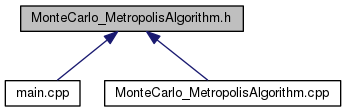
\includegraphics[width=332pt]{_monte_carlo___metropolis_algorithm_8h__dep__incl}
\end{center}
\end{figure}
\subsection*{Classes}
\begin{DoxyCompactItemize}
\item 
class \hyperlink{class_monte_carlo___metropolis_algorithm}{Monte\+Carlo\+\_\+\+Metropolis\+Algorithm}
\begin{DoxyCompactList}\small\item\em This class integrates a function using Metropolis sampling Brief description continued. \end{DoxyCompactList}\end{DoxyCompactItemize}

\hypertarget{_monte_carlo___uniform_sampling_8cpp}{}\section{Monte\+Carlo\+\_\+\+Uniform\+Sampling.\+cpp File Reference}
\label{_monte_carlo___uniform_sampling_8cpp}\index{Monte\+Carlo\+\_\+\+Uniform\+Sampling.\+cpp@{Monte\+Carlo\+\_\+\+Uniform\+Sampling.\+cpp}}
{\ttfamily \#include $<$cmath$>$}\newline
{\ttfamily \#include $<$cstdlib$>$}\newline
{\ttfamily \#include $<$ctime$>$}\newline
{\ttfamily \#include $<$random$>$}\newline
{\ttfamily \#include $<$chrono$>$}\newline
{\ttfamily \#include \char`\"{}Monte\+Carlo\+\_\+\+Uniform\+Sampling.\+h\char`\"{}}\newline
Include dependency graph for Monte\+Carlo\+\_\+\+Uniform\+Sampling.\+cpp\+:\nopagebreak
\begin{figure}[H]
\begin{center}
\leavevmode
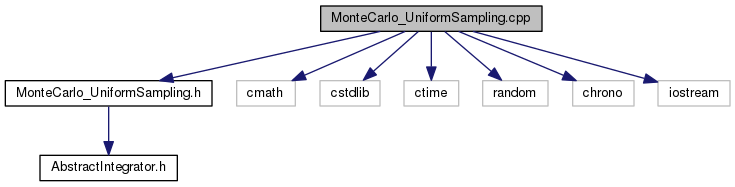
\includegraphics[width=350pt]{_monte_carlo___uniform_sampling_8cpp__incl}
\end{center}
\end{figure}

\hypertarget{_monte_carlo___uniform_sampling_8h}{}\section{/home/pcsc/\+P\+C\+S\+C2017\+\_\+\+Group2/\+Monte\+Carlo\+\_\+\+Uniform\+Sampling.h File Reference}
\label{_monte_carlo___uniform_sampling_8h}\index{/home/pcsc/\+P\+C\+S\+C2017\+\_\+\+Group2/\+Monte\+Carlo\+\_\+\+Uniform\+Sampling.\+h@{/home/pcsc/\+P\+C\+S\+C2017\+\_\+\+Group2/\+Monte\+Carlo\+\_\+\+Uniform\+Sampling.\+h}}
{\ttfamily \#include \char`\"{}Abstract\+Integrator.\+h\char`\"{}}\newline
Include dependency graph for Monte\+Carlo\+\_\+\+Uniform\+Sampling.\+h\+:
% FIG 0
This graph shows which files directly or indirectly include this file\+:
% FIG 1
\subsection*{Classes}
\begin{DoxyCompactItemize}
\item 
class \hyperlink{class_monte_carlo___uniform_sampling}{Monte\+Carlo\+\_\+\+Uniform\+Sampling}
\begin{DoxyCompactList}\small\item\em Brief description about the class. Brief description continued. \end{DoxyCompactList}\end{DoxyCompactItemize}

\hypertarget{_r_e_a_d_m_e_8md}{}\section{R\+E\+A\+D\+M\+E.\+md File Reference}
\label{_r_e_a_d_m_e_8md}\index{R\+E\+A\+D\+M\+E.\+md@{R\+E\+A\+D\+M\+E.\+md}}

%--- End generated contents ---

% Index
\backmatter
\newpage
\phantomsection
\clearemptydoublepage
\addcontentsline{toc}{chapter}{Index}
\printindex

\end{document}
